\section{(In)Comparability Graphs}
\label{tree:poset:graph}


\subsection{Definition}

We define the comparability graph ${G}(P)$ to be an undirected graph where all comparable elements in $P$ are represented as adjacent elements.

Similarly, we define the incomparability graph $\widetilde{G}(P)$ to be an undirected graph where all incomparable elements in $P$ are represented as adjacent elements.

By abuse of notation we write ${G}$ instead of ${G}(P)$.



\begin{figure}
	\centering
	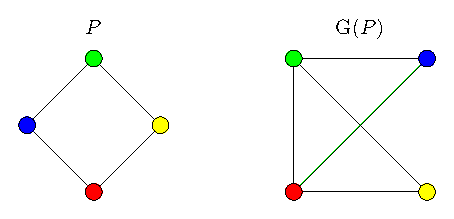
\includegraphics[width=0.6\textwidth]{fig/comp-graph}
	\caption{\label{fig:comp-graph} A Hasse Diagram and its comparability graph.}
\end{figure}




\subsection{Cliques and Stable Sets}

\defbox{A clique $C$ of graph $G$ is a subset of pairwise adjacent vertices in $G$, i.e. the subgraph induced by $C$ is complete.}

A clique in comparability graph ${G}$ is a subset of comparable  elements in ${P}$, i.e. a chain in ${P}$.

A clique in incomparability graph $\widetilde{G}$ is a subset of incomparable  elements in ${P}$, i.e. an antichain in ${P}$.

\defbox{A set $S$ is stable (or independent) if the vertices in $S$ are pairwise nonadjacent, i.e. the subgraph induced by $S$ has $\#S$ connected components.}

A stable set in comparability graph ${G}$ is a subset of incomparable elements in ${P}$, i.e. an antichain in ${P}$.

A stable set in incomparability graph $\widetilde{G}$ is a subset of comparable elements in ${P}$, i.e. a chain in ${P}$.


A stable set in ${G}$ is thus a clique in $\widetilde{G}$ and vice versa.



\subsection{$\operatorname{STAB}(G)$}


\begin{equation}
\operatorname{STAB}(G) := \operatorname{conv}\{\chi^S \in \mathbb{R}^V : S\text{ stable set in }G\}
\label{eq:stab}
\end{equation}

\ref{eq:stab} is the definition of the \emph{stable set polytope} of an arbitrary graph $G$ with vertex set $V = \left\{{v_1, \cdots, v_n }\right\}$ and order $n$ ($\mathbb{R}^V = \mathbb{R}^n, n = \#V$) i.e. the convex hull (an $n$-dimensional polytope) of stable set characteristic vectors $\chi^S \in \mathbb{R}^n$ where

$$ \chi^S_v =\begin{cases}
      1, & \text{if}\ v \in S\\
      0, & \text{otherwise}
    \end{cases}$$



\subsection{Entropy for Comparability Graphs}

In \ref{eq:entropy:graph} we find $x^*$ which minimize the average on $\log \frac{1}{x_v}$.

\begin{equation}
{H}(G) \coloneqq \min_{x \in \operatorname{STAB}(G)}~ -\frac{1}{n} \sum_{v \in V} \log x_v
\label{eq:entropy:graph}
\end{equation}



\subsection{Entropy for posets}


As we defined ${H}(G)$ in \ref{eq:entropy:graph}, we write ${H}(P)$ to mean ${H}(G(P))$.

\begin{equation}
{H}(P) \coloneqq {H}({G}(P))
\label{eq:entropy:poset}
\end{equation}
